\documentclass[11pt,a4paper,openany]{book}
\usepackage{preamble}
\usepackage{opstilling}
\usepackage{referencekommandoer}

\author{Mikkel B. Goldschmidt \\ 3r, Nørre Gymnasium \\ SRP i matematik og fysik}
\title{Dæmpede svingninger og differentialligninger}
\begin{document}
\maketitle
\tableofcontents

\chapter{Introduktion af problemet}
Jeg vil i denne opgave tage udgangspunkt i en bevægelse, som jeg vil forsøge at begrunde og beskrive. 
For at dette er muligt, er jeg dog nødt til kort at introducere en smule af pensum fra gymnasiet, som vil blive brugt i mine uledninger. 
Denne del af pensum vil jeg kun redegøre for, og jeg vil altså derfor ikke nødvendigvis efterprøve dem eksperimentielt eller forklare den mere teoretiske baggrund. 

\section{Nødvendig baggrundsteori}
\subsection{Hooks lov}\label{teori:Hooks lov}
Når man hiver i en fjeder, vil den have en kraft, modsatrettet den retning man hiver, der er proportional med hvor meget man har strukket fjederen\refFysA{286}. 
Dette giver anledning til formlen 
$$F =k\cdot x$$
hvor $x$ er den længde som fjederen er strukket, $F$ er kraften som fjedderen trækker med og $k$ er propertionalitetskonstanten. 
$k$ kaldes i denne sammenhæng for fjedderkonstanten.

\subsection{Newtons anden lov}\label{teori:Newtons anden lov}
Newtons anden lov fortæller ud fra den kraft et objekt påvirkes med og dets masse, hvor stor meget objektet vil accelerere. 
Den siger, at massen ganget med accelerationen af et objekt giver den kraft, som objektet bliver påvirket med\refFysA{217}.
\section{Forsøgsopsætning}
Hele denne opgave tager udgangspunkt i et forsøg.
I forsøget hænges et lod op i en fjeder der opfylder Hooks lov (se \ref{teori:Hooks lov}). 
Da tilføres loddet energi, således at det begynder at svinge. 
På figur \ref{fig:Basis Forsogsopsaetning} ses en skitse af forsøgets opsætning.

\begin{figure}[h]
\center
\opstilling{-1}%Se opstilling.sty i hovedmappen for definition. Ser bedst ud med udgangsposition i -1.

\caption{Skitse af forsøgsopsætning.}
\label{fig:Basis Forsogsopsaetning}
\end{figure} 

\subsection{Teoretiske egenskaber for bevægelsen}
Man kan da overveje, hvilke kræfter der påvirker loddet. 
Det er klart at loddet er påvirket af en tyngdekraft. 
Derudover er loddet påvirket af kraften fra fjederen.
Til sidst vil loddets bevægelse også være påvirket af luften omkring den hvis loddet er sat i bevægelse. 
Jeg vil starte med at kigge på, hvordan loddet vil opføre sig hvis man ser på en forholdsvist langsom bevægelse i en kortere tidsperiode.
Da kan vi nemlig se bort fra luftens dæmpning. 

\subsubsection{Differentialligning uden dæmpning}\label{teori: Opstilling ligning uden dampning}
Hvis vi betragter opadgående retning som værende positiv retning, kan vi altså opskrive den resulterende kraft på loddet som $F_{res} = F_{fjeder}-F_{t}$, hvor $F_t$ betegner tyngdekraften på loddet. 
Men vi kan da omskrive til en differentialligning ved at udnytte at $F_{fjeder}=k \cdot x(t)$ (se \ref{teori:Hooks lov}) hvor $x(t)$ er en funktion der beskriver loddets højde i forhold til et udgangspunkt (typisk vil dette udgangspunkt være den højde vil være i når det hænger stille). 
Derudover kan vi udnytte $F_{t}=m\cdot g$ hvor $m$ beskriver loddets masse og $g$ tyngdeaccelerationen. 
Til sidst ved vi fra Newtons anden lov (se \ref{teori:Newtons anden lov}) at $F_{res}=m\cdot a(t) = m \cdot x''(t)$ 
(her er udnyttes at accelerationen af et objekt er lig dets stedfunktion differentieret dobbelt\refFysA{187}). 
Dermed får vi altså ligningen :
$$m\cdot x''(t)=k\cdot x(t)-mg$$ 
som vi ser er en differentialligning i $x(t)$.

\subsubsection{Differentialligning med dæmpning}\label{teori: Opstilling af ligning med dampning}
Vi kan på samme måde som i forrige afsnit opskrive et udtryk der beskriver den resulterende kraft på loddet. 
Denne gang skal der bare trækkes et led mere fra på højresiden - nemlig luftmodstanden. 
Da vi i de fleste bevægelse tilnærmelsesvist kan beskrive luftmodstanden som værende proportional med hastigheden, kan vi skrive den som $- \mu x'(t)$ hvor $\mu$ er en proportionalitetskonstant og $x'(t)$ er stedfunktionen differentieret (og altså en beskrivelse af farten til tiden $t$\refFysA{187}).
her får vi altså en differentialligning på formen:
$$m\cdot x''(t)=-k\cdot x(t)-\mu x'(t) -mg$$
Fremover til $\mu x(t)$ blive omtalt som \textit{dæmpningsledet}, da det netop er luftmodstanden der gør at bevægelsen ikke bliver ved for evigt, da den giver anledning til en dæmpning. 

\chapter{Matematisk baggrund}
Før jeg forsøger at finde ud af hvordan forsøget forventes at forløbe i teorien, bliver jeg nødt til at have noget mere matematisk baggrund. 
Det er denne matematiske baggrund jeg vil forsøge at introducere i dette kapitel. 
Målet med hele kapitlet er at kunne finde den fuldstændige løsning til den generelle lineære homogene andenordens differentialligning samt at overveje hvad der sker hvis dæmpningsledet i denne bliver i anden potens i stedet for i første. 
\section{Den komplekse eksponentialfunktion}
I gymnasiet bliver man kort introduceret til de komplekse tal, og jeg tager derfor for givet, at læseren kan løse en andengradsligning, hvor diskriminanten er skarpt mindre end $0$ og derfor giver to komplekse løsninger. 
I gymnasiet lærer man dog ikke, at kunne opløfte tal i komplekse tal. 
Dette er dog en nødvendighed at kunne i denne opgave. 
Jeg vil derfor introducere definitionen af eksponentialfunktionen defineret på de komplekse tal $\mC$. 
Jeg vil ikke argumentere for, at denne opfører sig som den konventionelle definition med $\mR$, men bare lave en reference til en note fra DTU hvor dette kan ses. 

\begin{definition}[Den komplekse eksponentialfunktion]\label{def: Den komplekse eksponentialfunktion}

Lad $z=a+bi$ være et vilkårligt komplekst tal. Vi kalder da den komplekse eksponentialfunktion for $exp_\mC$. 
Vi definerer da denne til at være lig $exp_\mC (z)=e^{a} \cdot (cos(b) + sin(b)i)$.
Hvor $e$ er Eulers tal. 
\end{definition}

\begin{thm}\label{thm: expC = e^x}
$exp_\mC (x) = e^x$ hvis $x$ er et reelt tal. 
\end{thm}

\begin{proof}
Dette ses ret tydeligt ved at sætte $x+0i$ ind i definitionen af $exp_\mC$, der da vil blive $$exp_\mC(x) = e^x \cdot (cos(0)+sin(0)i)=e^x \cdot 1 = e^x \hspace{3cm}
\text{(Da $\sin (0)=0$ og $\cos (0)=1$)}$$
Dermed vist $exp_\mC (x) = e^x, \forall x \in \mR$
\end{proof}

\begin{thm}[Regneregler for $\exp_\mC$]\label{thm: regneregler for expC}
Følgende regneregler gælder for den komplekse eksponentialfunktion:
\begin{enumerate}
	\item $\eC (0)=1$
	\item $\eC (z_1+z_2) = \eC (z_1) \cdot \eC(z_2)$ for alle komplekse tal $z_1$ og $z_2$
	\item $(\eC (z))^n = exp_C (zn)$ for alle $n\in \mN$ og $z \in \mZ$.
\end{enumerate}
\end{thm}

\begin{proof}
Beviset for sætning \ref{thm: regneregler for expC} er ikke medtaget her grundet mangel på plads. Det kan læses i DTU's note om komplekse tal\refDTUKompleks{29.44}. 
\end{proof}

Vi kan se, at $\eC$ opfører sig på mange måder på samme måde som $e^x$, og specielt fordi $\eC$ altid tager de samme værdier som $e^x$ hvor den er defineret (de reelle tal, se sætning \ref{thm: expC = e^x}), tillader vi os fremover, at lade $e^x$ beskrive $\eC (x)$, og dermed er $e^x$ altså nu defineret fra $\mC$ over i $\mC$.
\section{Den andenordens lineære homogene differentialligning}
Det store problem i denne opgave er at bestemme den fuldstændige løsning til differentialligningerne der er beskrevet i afsnit \ref{teori: opsatning af differentialligninger}.
Disse er kan begge beskrives på formen $y'' + by' + cy = 0$, hvor $b,c \in \mR$ og $y$ er en differentialbel funktion fra de reelle tal over i de reelle tal. 
Bemærk her at der ikke er et konstantled foran $y''$. 
Dette gør ikke at vi mister generalitet, da vi altid ville kunne dividere hele ligningen igennem med den konstant der havde stået foran $y''$, og vi ville da have fået det på den ovenstående form. 
Jeg vil i dette afsnit bestemme den fuldstændige løsning til denne ligning. 
Mine udledninger her er stærkt inspirerede af Kalkulus\refKalkulus{529-539}. 

Jeg vil først vise et lemma der vil gøre mine udregninger nemmere senere.

\begin{lemma}
Hvis $g$ og $h$ er løsninger til den lineære andenordens differentialligning, da er $y(x) = C\cdot g(x) + D \cdot h(x)$ også en løsning for alle reelle konstanter $C,D$. 
\end{lemma}

\begin{proof}
Antag af $h$ og $g$ er løsninger til den lineære andenordens differentialligning. 
Vi starter med at indse at $y'=Cg' + Dh'$ og $y'' = Cg'' + Dh''$, ved brug af normale regler for differentiation. 

Vi betragter da ligningen med $y$ indsat:
\begin{align*}
y'' + by' + cy 	&= (Cg'' + Dh'') + b(Cg' + Dh') + c(Ch + Dh)	& \text{(Egenskaberne beskrevet ovenfor)}\\
				&= Cg'' + Dh'' + bCg' + bDh' + cCh + cDh		\\
				&= C(g'' + bg' + cg) + D(h'' + b'h + ch)		& \text{(Sætter udenfor parantes)}\\
				&= C\cdot 0 + D \cdot 0							& \text{(Udnytter at $g$ og $h$ er løsninger)}\\
				&= 0 
\end{align*}
Da kan vi ses at $y'' + by' + cy = 0$, dermed er $y$ er løsning til differentialligningen.
\end{proof}

Når vi snakker om lineære andenordens differentialligninger, er koefficienterne helt centrale for den fuldstændige løsning. 
Det vil vise sig senere, at en tilhørende andengradsligning til en lineær andenordens differentialligning, er helt central. Vi kalder denne for den \textit{Karakterligningen}.

\begin{definition}[Karakterligningen]
Karakterligningen for en lineær andenordens differentialligning $y'' + by' + cy = 0$, er ligningen $r^2 + br + c = 0$. 
Denne ligning har som bekendt en eller to komplekse løsninger $r_1 = \frac{-b + \sqrt{b^2 - 4c}}{2}$ og $r_2 = \frac{-b - \sqrt{b^2 - 4c}}{2}$. 
Fremover vil $r_1$ og $r_2$ referere til disse to definitioner af løsninger af karakterligningen for en given lineær andenordens differentialligning.

\end{definition}
\subsection{To komplekse rødder i karakterligningen}
\label{teori: Komplekse losninger i karakterligningen}
Jeg vil ikke føre fuldstændigt bevis for den fuldstændige løsning, når løsningerne til karakterligningen er komplekse. 
Dette gør jeg ikke fordi at beviset minder meget om beviset for sætning \ref{thm: fuldstandig losning}.

Man kunne formode ud fra sætning \ref{thm: fuldstandig losning}, at løsningerne ville være på formen $C\cdot e^{r_1 x} + D \cdot e^{r_2 x}$.
Her bliver vi dog nødt til først at bemærke noget om $r_1$ og $r_2$.
Vi ved at disse to er løsninger til den samme andengradsligning, og dermed må de også være komplekst konjugerede af hinanden\refKalkulus{133}. 
Dermed må vi kunne skrive dem som $r_1 = a + bi$ og $r_2 = a-bi$. 
Man kunne derfor tænke, at løsningen til den lineære andenordens differentialligning ville være på formen $C\cdot e^{(a+bi) x} + D \cdot e^{(a-bi)x}$.
Dette kan vi dog skrive om med definition \ref{def: Den komplekse eksponentialfunktion} til $Ce^{ax}(\cos(bx) + \sin(bx) i) + De^{ax}(\cos(-bx) + \sin(-bx) i)$.
Vi kan da flytte $e^{a}$ udenfor parentes og få 
$e^{ax}(C(\cos(bx) + \sin(bx) i) + D(\cos(-bx) + \sin(-bx) i))$.
Da det gælder om cosinus og sinus at $\cos(-x)=\cos(x)$ og $\sin(-x)=-\sin(x)$, kan vi videre omskrive til 4
$e^{ax}(C(\cos(bx) + \sin(bx) i) + D(\cos(bx) - \sin(bx) i))$. 
Dette kan ved brug af additionsformlen for sinus omskrives videre til $e^{ax}\cdot \sqrt{C^2 + D^2}\sin(bx+\phi)$. 
Jeg vil ikke føre et argument for den sidste omskrivning.
Dette skyldes at der kræves en forholdvist dybdegående forståelse for de trigonometriske funktioner for at kunne gennemføre argumentet. 
Argumentet for omskrivningen kan ses i Kalkulus\refKalkulus{538-539}.

Man kan argumentere for at mængden af alle funktioner på den før omtalte form er den fuldstændige løsning til den lineære andenordens homogene differentialligning når den har komplekse rødder i sin karakterligning. 
Jeg vil dog udelade beviset, da det føres på næsten samme måde som beviset for sætning \ref{thm: fuldstandig losning}. 

Jeg har altså den fuldstændige løsning til differentialligningen (når rødderne er komplekse) som:
$y(x) = e^{ax}\sqrt{C^2 + D^2}\sin(bx+\phi)$, i fysiksammehænge sætter vi dog ofte $\sqrt{C^2 + D^2}$ til at være lig med en konstant $A$, da denne viser sig at være en amplitude. 
Vi har derfor løsningerne på formen:
$$y(x) = e^{ax}A\sin(bx+\phi)$$



\subsection{Den ikke-lineære andenordens homogene differentialligning}
\label{teori: Den ikke-linear andenordens ligning}
I det vi indtil videre kun har kigget på den andenordens \textit{lineære} \textit{homogene} differentialligning, har vi lavet nogle antagelser som gør matematikken pæn, men disse holder dog ofte ikke i fysikkens verden.
Hvis man ser tilbage på afsnit \ref{teori:vindmodstand} om vindmodstand, har vi faktisk kun lavet matematisk teori der beskriver bevægelse ved lave hastigheder, da vi kun har kigget på når dæmpningsledet er i første. 
I afsnittet er det også beskrevet hvordan man ved høje hastigheder nærmere får at vindmodstanden er i anden.
Dette ville give anledning til en differentiallligning på formen:
$$y'' + b(y')^2 + cy = 0$$
Denne ligning er altså stadig homogen da den er lig med $0$, men ikke længere lineær. 
Det viser sig dog, at dette problem er markant sværere at løse end da dæmpningsledet var i første. 
Hvis vi kigger tilbage på beviset for sætning \ref{thm: fuldstandig losning}, så er det der fungerer i beviset at vi kan få hevet karakterligningen ud ved omskrivninger. 
Dette er kun muligt fordi alle tre led står i første. 
Havde vi forsøgt samme trick i den ikke-lineære, ville vi have fået en forkert potens på løsningen og dermed havde vi ikke kunnet nå i mål med beviset. 

Man kunne derfor prøve at løse den med et CAS-værktøj. 
Ved brug af Maple får jeg to løsninger (en med positivt og en med negativt fortegn, se $\pm$):
$$\int ^{y \left( x \right) }\!\pm 2\,{\frac {b}{\sqrt {4\,{{\rm e}^{-2\,b{
\it a}}}{\it C_1}\,{b}^{2}-4\,c{\it a}\,b+2\,c}}}{d{\it a}}-x-{
\it C_2}=0 \text{ hvor } C_1,C_2 \in \mR
$$
Dette har vi ikke redskaberne til at forstå med gymnasiepensum. 
For så vidt giver integralet og de to konstanter mening, men det at der kun er en øvre grænse og at grænsen er den funktion vi forsøger at finde, gør at dette nok ikke er en farbar vej til til at finde en løsning. 

Derfor er der nok kun vejen frem at løse problemet numerisk. 
Ved en numerisk løsning af en differentialligning, forstås at man kender en værdi på grafen og beregner flere værdier ud derfra.
Dog skal man når man regner på andenordens differentialligninger kende en sammenhørende værdi af $y$, $y'$ eller $y''$ for at kunne give et entydigt svar\refKalkulus{539}.
Jeg vil forsøge at lave en numerisk løsning senere, når jeg skal behandle data fra mine forsøg. 


\chapter{Forsøg}
Hele denne opgave tager udgangspunkt i et forsøg.
Jeg vil her beskrive dette forsøg, og udnytte den matematik, jeg har beskrevet, til at finde ud af om de opstillede differentialligninger fra afsnit \ref{teori: opsatning af differentialligninger} rent faktisk passer på virkeligheden.

Jeg har udført to forsøg, som hvert især er tænkt til at afprøve et stykke teori:
\begin{itemize}
	\item Svingning af lod i luft i kort tid
	\item Svingning af lod i luft i længere tid
\end{itemize}

Det første forsøg er ment til, at skulle passe på differentialligningen uden dæmpningsled.

Det andet forsøg er tænkt til at passe med et dæmpningsled ved lav fart, og altså derfor med dæmpningsledet i 1. potens.
Dette forsøg undersøger også om en model med dæmpningsledet i anden potens vil fungere bedre, end en med leddet i første potens.  

\section{Forsøg: Svingning af lod i luft i kort tid}

\subsection{Forsøgsbeskrivelse}\label{exp1: Beskrivelse af experiment}
\subsubsection{Materialer}
\begin{wrapfigure}{r}{0.4\textwidth}
\centering
\opstillingEt{-1}%Se opstilling.sty i hovedmappen for definition. Ser bedst ud med udgangsposition i -1.

\caption{Skitse af forsøgsopsætning til forsøg 1. Den grå figur under loddet er en ultralydsensor.}
\label{fig:Forsogsopsaetning 1}
\end{wrapfigure} 

Disse materialer blev brugt til forsøget:
\begin{itemize}
	\setlength\itemsep{-1em}
	\item Lod
	\item Fjeder
	\item Kraftmåler
	\item Tavlelineal ($1$ meter)
	\item Stativ til opsætning
	\item Ultralydsensor
	\item Computer til opsamling af data
\end{itemize}

\subsubsection{Udførelse}



Før selve udførslen af forsøget, bestemmer jeg en fjederkonstant for den fjeder jeg arbejder med. 
Dette gøres ved at måle samhørende værdier at udstrækning af fjederen og hvor stor en kraft den trækker med. 

I dette forsøg har jeg opsat et lod i en fjeder, som set på figur \ref{fig:Forsogsopsaetning 1}.
Derefter har jeg sat loddet i svingninger og målt loddets position med ultralydsensoren i en periode på $10$ sekunder. 
Jeg gentog dette forsøg 10 gange. 


\subsection{Hypotese}\label{exp1: Hypotese}
Da dette forsøg forløber over forholdsvist kort tid, forventer jeg at man betragte denne bevægelse som om den ikke er dæmpet, da dæmpningsledet vil være forholdvist småt. 
Dermed forventes differentialligningen 
$$m\cdot x'' = -k \cdot x$$
at være opfyldt, jvf. afsnit \ref{teori: Opstilling ligning uden dampning}.
Dette kan omskrives til $m\cdot x'' + k\cdot x=0$, hvilket vi ser er en andenordens lineær homogen differentialligning. 
Vi kan derfor bestemme en karakterligning som $mr^2 + k = 0 \Rightarrow r^2 + \frac{k}{m} = 0$ og dermed får vi $r = \frac{\pm \sqrt{-4\frac{k}{m}}}{2}=\pm\sqrt{\frac{k}{m}}i$.
Dermed skal vi have fat i den løsning af differentialligningen hvor løsningerne til karakterligningen er komplekse. 
Vi får da at løsningen skal være på formen (se afsnit \ref{teori: Komplekse losninger i karakterligningen}:
$$y(x) = e^{ax}A\sin(bx+\phi) \text{ hvor rødderne i karakterligningen er } r = a \pm bi$$
Vi ser dog her at rødderne i vores karakterligning ikke har nogen realdel, og dermed får vi at $e^{ax}=e^{0x}=1$.
Da $b=\sqrt{\frac{k}{m}}$ forventer vi derfor at bevægelsen vil kunne beskrives som 
$$x(t)=A\sin (\frac{k}{m}t+\phi)$$
hvor $\phi$ er en eller anden konstant. 


\subsection{Data}\label{exp1: Data}
\subsubsection{Svingning}
Data til dette forsøg er vedlagt som bilag i filen ''Forsøg 1 - Data.pdf''
Denne fil indeholder alt rådata opsamlet af ultralydsensoren i de 10 forsøg (OBS. filen er $130$ sider lang da der er blevet opsamlet $40$ målinger i sekundet). 
Forsøg nummer 10 er placeret først grundet måden mit dataopsamlingsprogram fungerer på.

\subsubsection{Fjederkonstant}\label{exp1: Fjederkonstant}
Ydermere er der vedlagt en fil ved navn ''Forsøg 1 og 2 fjederkonstant - Data.pdf''.
Denne fil indeholder data til bestemmelse af fjederkonstanten. 

\subsubsection{Masse af fjeder og lod}\label{exp1: Masse af fjeder og lod}
Jeg har målt massen af lodet og af fjederen i forbindelse med forsøget. 
Disse to er nedskrevet i tabel \ref{tabel: Masser forsog 1}.
\begin{table}[h]
\centering
\begin{tabular}{|c|c|}
\hline 
 & Masse ($g$) \\ 
\hline 
Fjeder & $77.09$ \\ 
\hline 
Lod & $32.45$ \\ 
\hline 
\end{tabular} 
\caption{Relevante masser til forsøg 1.}
\label{tabel: Masser forsog 1}
\end{table}

\subsection{Databehandling}\label{exp1: databehandling afsnit}
\subsubsection{Fjederkonstant}\label{databehandling: tyk fjeder fjederkonstant}
For at finde en fjederkonstant for fjederen der bliver brugt til forøget, har jeg taget de sammenhørende værdier af fjederkraft og udstrækning og plottet dem i kraft som afhængig og udstrækning som uafhængig variabel. 
Derefter har jeg lavet en best-fit lineær sammenhæng. 
Denne havde en forholdsvist lav RMSE på $0.044N$, og derfor virker dataen pålidelig. 
Vi må da have fjederkonstanten som hældningen på dette plot, i dette tilfælde $3.6\frac{N}{m}$.

Den tilhørende graf samt best-fit plot kan ses i bilaget "Forsøg 1 - grafer.pdf". 
 

\subsubsection{Best-fit kurver}\label{exp1: Best-fit kurver}
For at tjekke hvor godt hypotesen holder, vil jeg forsøge at lægge få min computer til at lave en best-fit kurve udfra funktionen $x(t)=A\sin (\sqrt{\frac{k}{m}}+\phi) + s_0$.
Det tilføjede $s_0$ for enden skyldes at loddet har hængt en afstand over ultralydsensoren som der skal justeres for. 

I tabel \ref{tabel: bestfitkurver forsog 1} kan ses værdier for $A, \sqrt{\frac{k}{m}}, \phi ,s_0$ og så den gennemsnitlige afvigelse målt i meter (RMSE).


\begin{table}[h]
\centering
\begin{tabular}{|l|c|c|c|c|c|}
\hline
\textbf{}          & \textbf{A}($m$) & \textbf{$\sqrt{\frac{k}{m}}$}($s^{-1}$) & \textbf{$\phi$} & \textbf{$s_0$}($m$) & \textbf{RMSE }($m$) \\ \hline
\textbf{Forsøg 10} & 0,08854    & 7,73                          & 584,8           & 0,2929         & 0,003136      \\ \hline
\textbf{Forsøg 1}  & 0,04319    & 7,632                         & 6,99            & 0,2984         & 0,001839      \\ \hline
\textbf{Forsøg 2}  & 0,06744    & 7,669                         & 20,9            & 0,2963         & 0,001766      \\ \hline
\textbf{Forsøg 3}  & 0,07559    & 7,692                         & 38,58           & 0,2948         & 0,002061      \\ \hline
\textbf{Forsøg 4}  & 0,081      & 7,707                         & -1,786          & 0,2933         & 0,003476      \\ \hline
\textbf{Forsøg 5}  & 0,08944    & 7,734                         & -1,145          & 0,2936         & 0,004427      \\ \hline
\textbf{Forsøg 6}  & 0,08174    & 7,709                         & 3,467           & 0,294          & 0,00381       \\ \hline
\textbf{Forsøg 7}  & 0,06552    & 7,663                         & 818,2           & 0,2954         & 0,001818      \\ \hline
\textbf{Forsøg 8}  & 0,05712    & 7,648                         & 9,939           & 0,2965         & 0,001589      \\ \hline
\textbf{Forsøg 9}  & 0,04544    & 7,633                         & 9,7             & 0,297          & 0,001462      \\ \hline
\end{tabular}

\caption{De forskellige værdier på best-fit kurver. De tilhørende grafer til dataen samt best-fit-plot er vedlagt som bilag i filen ''Forsøg 1 - grafer.pdf''}
\label{tabel: bestfitkurver forsog 1}
\end{table}

\subsubsection{Teoretisk bestemmelse af loddets masse}\label{exp1: teoretisk bestemmelse af loddets masse}

\subsubsection{Vurdering af data}\label{exp1: Vurdering af data}
Det første der er værd at bemærke, er at værdierne af $\sqrt{\frac{k}{m}}$ ligger meget tæt på hinanden. 
Dette stemmer godt overens med teorien da denne værdi ikke bør være afhængig af hvor meget der energi der bliver tilførst systemet til at starte med, men kun hvilken masse lodet har og hvilken fjederkonstant fjederen har. 
Da forsøget er lavet med samme fjeder og samme lod, må man forvente samme værdi, hvilket også er det vi observerer, da der kun er en forskel på $7.734s^{-1}-7.632s^{-1}=0.102s^{-1}$ på den største og mindste værdi, hvilket er relativt lidt i forhold til de ca. 7 en halv tallene ligger på.



Derudover er det værd at bemærke de meget lave afvigelser. 
Den gennemsnitlige afvigelse ligger imellem $0.3136cm$ og $0.4427cm$ i forhold til amplituder på helt op til $8.944cm$. 
Dette må anses som forholdsvist små afvigelser i forhold til hele bevægelsen.


\subsection{Konklusion}



\section{Forsøg: Svingning af lod i luft i længere tid}

\subsection{Forsøgsbeskrivelse}
Dette forsøg forløber nøjagtigt på samme måde som forsøg 1 (se forsøgsbeskrivelse \ref{exp1: Beskrivelse af experiment})


\subsection{Hypotese}

\subsection{Data}

\subsection{Databehandling}

\subsection{Konklusion}



\section{Forsøg: Svingning af lod i vand}

\subsection{Forsøgsbeskrivelse}

\subsection{Hypotese}

\subsection{Databehandling}

\subsection{Konklusion}




\chapter{Perspektivering - Affjedring af biler}
Den harmoniske svingning optræder mange andre steder i mekanikken end bare når et lod svinger i en fjeder.
Det ses blandt i forbindelse med penduler og generet med ting der drejer rundt.
Derudover er det også relevant at kigge på i forbindelse med større bygninger som eksempelvis broer, der kan gå i svingninger hvis de ikke er konstrueret rigtigt. 

Et andet sted hvor man kan se svingninger af fjedre meget markant er i forbindelse med affjedring af biler. 
Det er nemlig sådan at en bils hjul er forbundet til fjedre. 
En skitse af dette kan ses på figur \ref{fig: Affjedring af bil}.

\begin{wrapfigure}{r}{0.4\textwidth}
\center
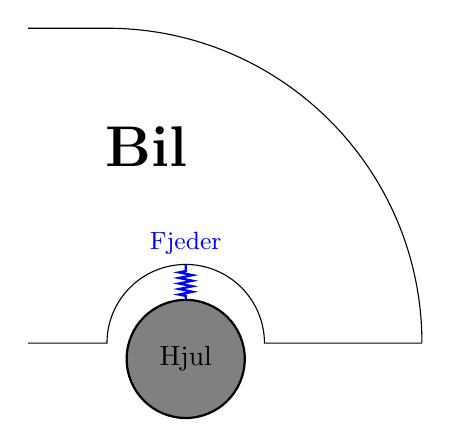
\begin{tikzpicture}
\tikzstyle{spring}=[thick,decorate,decoration={zigzag,pre length=0.05cm,post length=0.05cm,segment length=2}]

\draw (-2,0)--(-1,0)--(-1,0) arc [radius=1, start angle=180, end angle= 0]--(1,0)--(3,0);%Bund af bil uden hjul

\draw (3,0) arc [radius=4, start angle=0, end angle = 90] -- (-2,4) ;%Top af bil

\draw[fill=gray, thick] (0,-0.2) circle (0.75) node {Hjul};%hjulet
\node at (-0.5,2.5) {\huge \textbf{Bil}};
\draw[spring, blue] (0,0.55)--(0,1) node[above, blue] {\small Fjeder};

\end{tikzpicture}
\caption{Skitsetegning af fjeder (blå) fastsat til bils hjul.}
\label{fig: Affjedring af bil}
\end{wrapfigure}

Fjederen er til for at sørge for at bilen hele tiden fastholder kontakt med vejen - også selvom den kører over en ujævnhed i vejen. 
Hvis fjederen går i stykker, kan det være meget problematisk. 
Der kan ske det, at fjederen dæmper for langsomt og at man derfor oplever at bilen hopper.
En video af af dette kan ses på YouTube\refBilVideo.
Som det ses på videoen, så bliver bilen ved med at svinge efter at manden har givet slip. 
Hvis man betragter denne svingning med den teori der er beskrevet i denne opgave, så svarer bilen til vores lod.
Vi er da interesserede i at få svingningen af bilen til at dø ud så hurtigt som muligt. 
Her arbejder vi ikke med luftmodstand, men derimod med en mekanisk dæmpning. 
Hvis vi antager at svingningen dæmpes på en måde, således at dæmpningen er proportional med hastigheden af svingningen med en proportionalitetskonstant $\xi$, har vi igen en lineær andenordens homogen differentialligning
$$mx''(t)+\xi x'(t) + k x(t) = 0$$
hvor $k$ er fjederkonstanten for bilens fjeder, $m$ er bilens masse og $x$ er en funktion af tiden der beskriver hvor højt/lavt bilen befinder sig i forhold til sit udgangspunkt.

Da vi er interesserede i at bilen hopper så lidt som muligt, er vi ikke interesserede i en harmonisk svingning. 
Vi ved fra teorien tidligere at der opstår en harmonisk svingning når rødderne i karakterligningen er komplekse. 
Derfor er man interesserede i at få en god nok kombination af dæmpningskonstant og fjederkonstant til at rødderne i karakterligningen ikke bliver komplekse. 

Vi vil derfor gerne prøve at kigge på karakterligningen. 
Vi får da en ligning $mr^2 + \xi r + k = 0$ hvilket giver os løsningerne (med andengradslignings løsningsformel):
$$r = \dfrac{-\xi \pm \sqrt{\xi ^2 - 4mk}}{2m}$$

For at vi ikke får komplekse rødder skal vi altså have at størrelsen $\xi ^2 -4mk$ er ikke-negativ, og det skal altså gælde at $0 \leq \xi ^2 -4mk $ eller omskrevet at $4mk \leq \xi ^2 $.
Her fra er man dog nødt til at vide mere omkring biler og kunne foretage nogle eksperimenter for at kunne fortsætte. 
Vi ved nemlig intet om $\xi$ og om hvordan dæmpning skabes. 

I forhold til videoen, kan vi se at bilen lige pludselig svinger og at karakterligningen derfor må have komplekse løsninger.
Vi ved derfor at der er sket en ændring af $k,m$ og $\xi$ sådan at det ikke længere gælder at $4mk \leq \xi ^2 $.
Da bilens masse, $m$, formentlig ikke har ændret sig, må vi altså enten have at $k$ er blevet større eller at $\xi$ er blevet mindre. 
Oversat til fysik, har vi altså enten at fjederen er blevet mere hård og derfor har en højere fjederkonstant eller at dæmpningssystemet ikke fungerer som det skal.  



\begin{thebibliography}{9}

%\bibitem{Bog_hele bogen}
%  Forfatter,
%  (Årstal, s. ...). 
%  Titel (Udgave). 
%  By,
%  Forlag

 
\bibitem{FysikA}
  Knud Erik Nielsen og Esper Fogh,
  (2007, s. 187-195). 
  Vejen til fysik A2 (1. udgave). 
  Silkeborg,
  Forlaget Hax

  
  
\end{thebibliography}


\end{document}
